% defer/rcufundamental.tex

\subsection{RCU Fundamentals}
\label{sec:defer:RCU Fundamentals}
\OriginallyPublished{Section}{sec:defer:RCU Fundamentals}{RCU Fundamentals}{Linux Weekly News}{PaulEMcKenney2007WhatIsRCUFundamentally}

Authors: Paul E. McKenney and Jonathan Walpole

Read-copy update (RCU) 는 2002년 10월에 리눅스 커널에 추가된, 하나의 동기화
메커니즘입니다.
RCU 는 읽기 작업들이 업데이트 작업들과 동시에 일어날 수 있도록 함으로써 확장성
개선을 달성합니다.
기존에 일반적으로 사용되어온, 동시에 수행되는 쓰레드들에 대해 그것들이 읽기를
하는지 업데이트를 하는지와 상관없이 상호 배제를 보장하는 락킹 기능들 또는
동시의 읽기 작업은 허용하지만 업데이트가 함께 수행되는 것은 막는 reader-writer
락들과는 대조적으로 RCU 는 하나의 업데이트 쓰레드와 여러 읽기 쓰레드들 사이의
동시성을 지원합니다.
RCU 는 오브젝트들의 여러 버전들을 유지하고 그것들이 이전부터 존재해온 모든
읽기쪽 크리티컬 섹션들이 완료되기 전까지는 메모리에서 해제하지 않음으로써 읽기
작업들이 일관적임을 보장합니다.
RCU 는 오브젝트의 새 버전을 공개하고 읽는데, 그리고 예전 버전들의 정리 작업을
뒤로 미루어 한번에 처리하는데에 효과적이고 확장성 있는 메커니즘을 정의하고
사용합니다.
이런 메커니즘들은 작업을 읽기와 업데이트쪽 수행경로로 분산시키되 읽기 쪽
수행경로가 극단적으로 빠르게 하는데에 해저드 포인터와 유사한 복사와 규칙 완화를
골자로 하는 최적화 기술을 사용하지만, 읽기 쪽의 재시도는 필요 없게 합니다.
일부 경우에는 (CPU 를 뺏기지 않는 커널들), RCU 의 읽기 쪽 기능들은 아예
오버헤드가 없습니다.
\iffalse

Read-copy update (RCU) is a synchronization mechanism that was added to
the Linux kernel in October of 2002.
RCU achieves scalability
improvements by allowing reads to occur concurrently with updates.
In contrast with conventional locking primitives that ensure mutual exclusion
among concurrent threads regardless of whether they be readers or
updaters, or with reader-writer locks that allow concurrent reads but not in
the presence of updates, RCU supports concurrency between a single
updater and multiple readers.
RCU ensures that reads are coherent by
maintaining multiple versions of objects and ensuring that they are not
freed up until all pre-existing read-side critical sections complete.
RCU defines and uses efficient and scalable mechanisms for publishing
and reading new versions of an object, and also for deferring the collection
of old versions.
These mechanisms distribute the work among read and
update paths in such a way as to make read paths extremely fast, using
replication and weakening optimizations in a manner similar to
hazard pointers, but without the need for read-side retries.
In some cases (non-preemptible kernels), RCU's read-side primitives have
zero overhead.
\fi

\QuickQuiz{}
	하지만 Section~\ref{sec:defer:Sequence Locks} 의 시퀀스 락 역시 읽기
	쓰레드들과 업데이트 쓰레드들이 동시에 일을 할 수 있도록 하지 않던가요?
	\iffalse

	But doesn't Section~\ref{sec:defer:Sequence Locks}'s seqlock
	also permit readers and updaters to get work done concurrently?
	\fi
\QuickQuizAnswer{
	맞는 말이고 아닌 말이기도 합니다.
	시퀀스 락의 읽기 쓰레드들은 쓰기 쓰레드들과 동시에 수행될 수 있지만,
	이런 상황이 발생할 때마다, {\tt read\_seqretry()} 기능이 읽기 쓰레드는
	다시 수행을 시도하도록 강제할 겁니다.
	이는 시퀀스 락을 사용하명 업데이트 쓰레드와 동시에 수행되는 읽기
	쓰레드가 하는 일은 모두 취소되고 다시 수행될 것을 의미합니다.
	따라서 시퀀스 락을 사용하는 읽기 작업은 업데이트 작업과 동시에
	\emph{수행} 될 수 있지만, 이런 경우에 실제로는 어떤 일도 만들어내지
	못합니다.

	반면에, RCU 읽기 쓰레드들은 동시에 RCU 업데이트 쓰레드들이 존재하더라도
	의미있는 일을 처리해낼 수 있습니다.
	\iffalse

	Yes and no.
	Although seqlock readers can run concurrently with
	seqlock writers, whenever this happens, the {\tt read\_seqretry()}
	primitive will force the reader to retry.
	This means that any work done by a seqlock reader running concurrently
	with a seqlock updater will be discarded and redone.
	So seqlock readers can \emph{run} concurrently with updaters,
	but they cannot actually get any work done in this case.

	In contrast, RCU readers can perform useful work even in presence
	of concurrent RCU updaters.
	\fi
} \QuickQuizEnd

이는 ``RCU 는 정확히 무엇인가?'' 하는 질문과, 아마도 ``RCU 는 어떻게 동작할 수
\emph{있는가}?'' 하는 질문을 이끌어낼 수 있을 겁니다 (또는, 드물지 않게, RCU 는
동작할 수 없을 것이라는 단정을).
이 문서는 이런 질문들을 기본적 관점에서부터 다룹니다; 뒤의 일부는 RCU 를
사용법과 API 관점에서 살펴봅니다.
마지막 부분은 또한 참고할 문서 목록을 포함합니다.

RCU 는 세개의 기본적 메커니즘으로 만들어지는데, 첫번째는 항목 삽입에 사용되고,
두번째 것은 항목 삭제에, 그리고 세번째 것은 읽기 쓰레드들이 동시의 항목 추가와
삭제에 문제 없이 동작하도록 하는데 사용됩니다.
Section~\ref{sec:defer:Publish-Subscribe Mechanism}
은 항목 추가를 위한 publish-subscribe 메커니즘을 설명하고,
Section~\ref{sec:defer:Wait For Pre-Existing RCU Readers to Complete}
에서는 먼저 시작된 RCU 읽기 쓰레드들을 어떻게 기다려서 항목 삭제가 가능하게
하는지 설명하며,
Section~\ref{sec:defer:Maintain Multiple Versions of Recently Updated Objects}
에서는 최근에 업데이트된 오브젝트들의 여러 버전들을 어떻게 관리해서 동시의 항목
추가와 삭제를 가능하게 하는지 설명합니다.
마지막으로,
Section~\ref{sec:defer:Summary of RCU Fundamentals}
에서는 RCU 기본사항을 요약합니다.
\iffalse

This leads to the question ``what exactly is RCU?'', and perhaps also
to the question ``how can RCU \emph{possibly} work?'' (or, not
infrequently, the assertion that RCU cannot possibly work).
This document addresses these questions from a fundamental viewpoint;
later installments look at them from usage and from API viewpoints.
This last installment also includes a list of references.

RCU is made up of three fundamental mechanisms, the first being
used for insertion, the second being used for deletion, and the third
being used to allow readers to tolerate concurrent insertions and deletions.
Section~\ref{sec:defer:Publish-Subscribe Mechanism}
describes the publish-subscribe mechanism used for insertion,
Section~\ref{sec:defer:Wait For Pre-Existing RCU Readers to Complete}
describes how waiting for pre-existing RCU readers enabled deletion,
and
Section~\ref{sec:defer:Maintain Multiple Versions of Recently Updated Objects}
discusses how maintaining multiple versions of recently updated objects
permits concurrent insertions and deletions.
Finally,
Section~\ref{sec:defer:Summary of RCU Fundamentals}
summarizes RCU fundamentals.
\fi

\subsubsection{Publish-Subscribe Mechanism}
\label{sec:defer:Publish-Subscribe Mechanism}

\begin{figure}[tbp]
{ \scriptsize
\begin{verbatim}
  1 struct foo {
  2   int a;
  3   int b;
  4   int c;
  5 };
  6 struct foo *gp = NULL;
  7
  8 /* . . . */
  9
 10 p = kmalloc(sizeof(*p), GFP_KERNEL);
 11 p->a = 1;
 12 p->b = 2;
 13 p->c = 3;
 14 gp = p;
\end{verbatim}
}
\caption{Data Structure Publication (Unsafe)}
\label{fig:defer:Data Structure Publication (Unsafe)}
\end{figure}

RCU 의 핵심 요소 중 하나는 데이터가 동시에 수정되고 있는데도 불구하고 안전하게
그 데이터를 읽을 수 있는 능력입니다.
동시의 항목 삽입에 이런 능력을 제공하기 위해, RCU 는 공개-구독
(publish-subscribe) 메커니즘이라 생각될 수 있는 방법을 상요합니다.
예를 들어, 초기에 \co{NULL} 인 전역 포인터 \co{gp} 가 새로 할당되고 초기화된
데이터 구조체로의 포인터로 수정되려 한다고 생각해 봅시다.
Figure~\ref{fig:defer:Data Structure Publication (Unsafe)} 에 보이는 코드 조각
(추가로 적절한 락킹을 포함해서) 이 이 목적으로 사용될 수 있을 것입니다.
\iffalse

One key attribute of RCU is the ability to safely scan data, even
though that data is being modified concurrently.
To provide this ability for concurrent insertion,
RCU uses what can be thought of as a publish-subscribe mechanism.
For example, consider an initially \co{NULL} global pointer
\co{gp} that is to be modified to point to a newly allocated
and initialized data structure.
The code fragment shown in
Figure~\ref{fig:defer:Data Structure Publication (Unsafe)}
(with the addition of appropriate locking)
might be used for this purpose.
\fi

안타깝게도, 컴파일러와 CPU 가 마지막 네개의 할당문이 순서대로 수행하도록
강제하는 것이 전혀 없습니다.
\co{gp} 로의 할당이 \co{p} 필드들의 초기화 전에 일어난다면, 동시 수행중인 읽기
작업들은 이 초기화되지 않은 값들을 볼 수 있을 겁니다.
이것들이 순서를 지키도록 하기 위해 메모리 배리어들이 필요합니다만, 메모리
배리어들은 사용하기가 어렵기로 악명높습니다.
따라서 그것들을 공개 의미를 갖는 \co{rcu_assign_pointer()} 기능에 집어넣습니다.
그렇게 되면 마지막 네줄은 다음과 같이 될겁니다:
\iffalse

Unfortunately, there is nothing forcing the compiler and CPU to execute
the last four assignment statements in order.
If the assignment to \co{gp} happens before the initialization
of \co{p} fields, then concurrent readers could see the
uninitialized values.
Memory barriers are required to keep things ordered, but memory barriers
are notoriously difficult to use.
We therefore encapsulate them into a primitive
\co{rcu_assign_pointer()} that has publication semantics.
The last four lines would then be as follows:
\fi

\vspace{5pt}
\begin{minipage}[t]{\columnwidth}
\scriptsize
\begin{verbatim}
  1 p->a = 1;
  2 p->b = 2;
  3 p->c = 3;
  4 rcu_assign_pointer(gp, p);
\end{verbatim}
\end{minipage}
\vspace{5pt}

이 \co{rcu_assign_pointer()} 는 새 구조체를 \emph{공개}하고, 컴파일러와 CPU 가
\co{gp} 로의 할당이 \co{p} 로 참조되는 필드들의 할당 \emph{후에} 수행하도록
강제할 겁니다.

하지만, 업데이트 작업에 순서를 맞추는 것만으로는 충분치 않은데, 읽기 작업도
적절하게 순서가 맞춰져야 하기 때문입니다.
다음과 같은 코드 조각의 예를 생각해 봅시다:
\iffalse

The \co{rcu_assign_pointer()}
would \emph{publish} the new structure, forcing both the compiler
and the CPU to execute the assignment to \co{gp} \emph{after}
the assignments to the fields referenced by \co{p}.

However, it is not sufficient to only enforce ordering at the
updater, as the reader must enforce proper ordering as well.
Consider for example the following code fragment:
\fi

\vspace{5pt}
\begin{minipage}[t]{\columnwidth}
\scriptsize
\begin{verbatim}
  1 p = gp;
  2 if (p != NULL) {
  3   do_something_with(p->a, p->b, p->c);
  4 }
\end{verbatim}
\end{minipage}
\vspace{5pt}

이 코드 조각은 잘못된 순서에 문제가 없을 것처럼 보이지만, 안타깝게도 DEC Alpha
CPU~\cite{PaulMcKenney2005i,PaulMcKenney2005j} 와 값을 예측하는 컴파일러
최적화는, 믿든 안믿든, \co{p->a}, \co{p->b}, 그리고 \co{p->c} 가 \co{p} 의 값
전에 메모리로부터 가져와질 수 있게 할 수 있습니다.
이런 현상은 컴파일러가 \co{p} 의 값을 추측하고 \co{p->a}, \co{p->b}, 그리고
\co{p->c} 값을 가져온 후에 그 추측이 맞았는지 보기 위해 \co{p} 의 실제 값을
가져오는, 컴파일러의 값 추측 최적화의 경우에서 보기가 가장 쉬울 겁니다.
이런 종류의 최적화는 상당히 공격적이고 미친 행위 같지만, 프로파일 기반의
최적화의 문맥에서는 실제로 일어나는 일입니다.
\iffalse

Although this code fragment might well seem immune to misordering,
unfortunately, the
DEC Alpha CPU~\cite{PaulMcKenney2005i,PaulMcKenney2005j}
and value-speculation compiler optimizations can, believe it or not,
cause the values of \co{p->a}, \co{p->b}, and
\co{p->c} to be fetched before the value of \co{p}.
This is perhaps easiest to see in the case of value-speculation
compiler optimizations, where the compiler guesses the value
of \co{p} fetches \co{p->a}, \co{p->b}, and
\co{p->c} then fetches the actual value of \co{p}
in order to check whether its guess was correct.
This sort of optimization is quite aggressive, perhaps insanely so,
but does actually occur in the context of profile-driven optimization.
\fi

분명히, 우리는 컴파일러와 CPU 로부터 이런 종류의 야바위질을 막아야 합니다.
\co{rcu_dereference()} 기능은 이런 목적을 위해 필요한 어떤 메모리 배리어
인스트럭션과 컴파일러 지시어들을 사용합니다:\footnote{
	리눅스 커널에서, \co{rcu_dereference()} 는 volatile 캐스팅으로
	구현되고, DEC Alpha 에서는 메모리 배리어 인스트럭션으로 구현됩니다.
	C11 과 C++11 표준에서는 \co{memory_order_consume} 이
	\co{rcu_dereference()} 지원을 제공하기 위한 의도로 만들어졌습니다만,
	이를 native로 구현한 컴파일러는 아직 없습니다.
	(컴파일러들은 대신 \co{memory_order_consume} 을
	\co{memory_order_acuire} 로 강화시켜서, 약한 순서 규칙의 시스템에서는
	필요없는 메모리 배리어 인스트럭션을 만듭니다.)}
\iffalse

Clearly, we need to prevent this sort of skullduggery on the
part of both the compiler and the CPU.
The \co{rcu_dereference()} primitive uses
whatever memory-barrier instructions and compiler
directives are required for this purpose:\footnote{
	In the Linux kernel, \co{rcu_dereference()} is implemented via
	a volatile cast, and, on DEC Alpha, a memory barrier instruction.
	In the C11 and C++11 standards, \co{memory_order_consume}
	is intended to provide longer-term support for \co{rcu_dereference()},
	but no compilers implement this natively yet.
	(They instead strengthen \co{memory_order_consume} to
	\co{memory_order_acquire}, thus emitting a needless memory-barrier
	instruction on weakly ordered systems.)}
\fi

\vspace{5pt}
\begin{minipage}[t]{\columnwidth}
\scriptsize
\begin{verbatim}
  1 rcu_read_lock();
  2 p = rcu_dereference(gp);
  3 if (p != NULL) {
  4   do_something_with(p->a, p->b, p->c);
  5 }
  6 rcu_read_unlock();
\end{verbatim}
\end{minipage}
\vspace{5pt}

따라서 \co{rcu_dereference()} 함수는 특정 포인터로 주어지는 값에 대한
\emph{구독} 으로, 뒤따르는 dereference 오퍼레이션들은 해당 포인터를 공개한,
연관된 \co{rcu_assign_pointer()} 오퍼레이션 전에 발생한 초기화 작업의 결과들을
보게 될 것이 보장된다고 이해될 수 있습니다.
\co{rcu_read_lock()} 과 \co{rcu_read_unlock()} 함수 호출들은 반드시 필요합니다:
이것들은 RCU read-side 크리티컬 섹션을 정의합니다.
이것들의 목적인
Section~\ref{sec:defer:Wait For Pre-Existing RCU Readers to Complete} 에서
설명됩니다만, 이것들은 결코 스피닝하거나 블락킹 하지 않고, \co{list_add_rcu()}
가 동시에 수행되는 것을 막지도 않습니다.
사실, \co{CONFIG_PREEMPT} 옵션이 켜져있지 않은 커널에서 이것들은 아무 코드도
생성하지 않습니다.
\iffalse

The \co{rcu_dereference()} primitive can thus be thought of
as \emph{subscribing} to a given value of the specified pointer,
guaranteeing that subsequent dereference operations will see any
initialization that occurred before the corresponding
\co{rcu_assign_pointer()} operation that published that pointer.
The \co{rcu_read_lock()} and \co{rcu_read_unlock()}
calls are absolutely required: they define the extent of the
RCU read-side critical section.
Their purpose is explained in
Section~\ref{sec:defer:Wait For Pre-Existing RCU Readers to Complete},
however, they never spin or block, nor do they prevent the
\co{list_add_rcu()} from executing concurrently.
In fact, in non-\co{CONFIG_PREEMPT} kernels, they generate
absolutely no code.
\fi

\begin{figure}[tb]
\begin{center}
\resizebox{3in}{!}{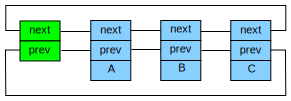
\includegraphics{defer/Linux_list}}
\end{center}
\caption{Linux Circular Linked List}
\label{fig:defer:Linux Circular Linked List}
\end{figure}

\begin{figure}[tb]
\begin{center}
\resizebox{3in}{!}{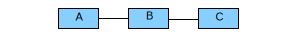
\includegraphics{defer/Linux_list_abbr}}
\end{center}
\caption{Linux Linked List Abbreviated}
\label{fig:defer:Linux Linked List Abbreviated}
\end{figure}

이론상으로는 \co{rcu_assign_pointer()} 와 \co{rcu_dereference()} 는 상상할 수
있는 RCU 로 보호되는 데이터 구조는 얼마든지 만들 수 있지만, 실제로는
고차원의 방법을 사용하는게 나은 경우가 많이 있습니다.
그런 이유로, \co{rcu_assign_pointer()} 와 \co{rcu_dereference()} 함수들이
리눅스에 있는 리스트 조정 API 의 특별한 RCU 사용 버전에 내장되어 있습니다.
리눅스는 이중 링크드 리스트의 두가지 버전을 가지고 있는데, 순환 형태의 {\tt
struct list\_head} 와 선형의 {\tt struct hlist\_head}/{\tt struct hlist\_node}
쌍입니다.
앞의 버전은
Figure~\ref{fig:defer:Linux Circular Linked List} 에 그려져 있는데, (왼쪽의)
초록 상자는 리스트 헤더를 나타내고 (오른쪽의 세개의) 파란 박스들은 리스트의
원소들을 의미합니다.
이 방법은 다루기가 힘들기 때문에
Figure~\ref{fig:defer:Linux Linked List Abbreviated} 에 보인 것처럼 헤더 없이
(파란) 원소들만을 보이는 형태로 간략화해서 나타낼 수 있습니다.
\iffalse

Although \co{rcu_assign_pointer()} and
\co{rcu_dereference()} can in theory be used to construct any
conceivable RCU-protected data structure, in practice it is often better
to use higher-level constructs.
Therefore, the \co{rcu_assign_pointer()} and
\co{rcu_dereference()}
primitives have been embedded in special RCU variants of Linux's
list-manipulation API.
Linux has two variants of doubly linked list, the circular
{\tt struct list\_head} and the linear
{\tt struct hlist\_head}/{\tt struct hlist\_node} pair.
The former is laid out as shown in
Figure~\ref{fig:defer:Linux Circular Linked List},
where the green (leftmost) boxes represent the list header and the blue
(rightmost three) boxes represent the elements in the list.
This notation is cumbersome, and will therefore be abbreviated as shown in
Figure~\ref{fig:defer:Linux Linked List Abbreviated},
which shows only the non-header (blue) elements.
\fi

\begin{figure}[tbp]
{ \scriptsize
\begin{verbatim}
  1 struct foo {
  2   struct list_head *list;
  3   int a;
  4   int b;
  5   int c;
  6 };
  7 LIST_HEAD(head);
  8
  9 /* . . . */
 10
 11 p = kmalloc(sizeof(*p), GFP_KERNEL);
 12 p->a = 1;
 13 p->b = 2;
 14 p->c = 3;
 15 list_add_rcu(&p->list, &head);
\end{verbatim}
}
\caption{RCU Data Structure Publication}
\label{fig:defer:RCU Data Structure Publication}
\end{figure}

이 링크드 리스트에 포인터 공개 예제의 기법을 적용하는 것은
Figure~\ref{fig:defer:RCU Data Structure Publication} 에 보여진 코드와 같은
형태로 귀결될 겁니다.

Line~15 는 여러개의 \co{list_add_rcu()} 가 동시에 수행되는 것을 막기 위해 어떤
다른 동기화 메커니즘 (가장 흔하게는 어떤 종류의 락) 을 사용해야만 합니다.
하지만, 그런 동기화는 이 \co{list_add()} 의 수행을 RCU 읽기 작업들과 동시에
수행되는 것을 못하게 하지는 않습니다.

RCU 로 보호되는 리스트를 구독하는 행위는 간단합니다:
\iffalse

Adapting the pointer-publish example for the linked list results in
the code shown in
Figure~\ref{fig:defer:RCU Data Structure Publication}.

Line~15 must be protected by some synchronization mechanism (most
commonly some sort of lock) to prevent multiple \co{list_add_rcu()}
instances from executing concurrently.
However, such synchronization does not prevent this \co{list_add()}
instance from executing concurrently with RCU readers.

Subscribing to an RCU-protected list is straightforward:
\fi

\vspace{5pt}
\begin{minipage}[t]{\columnwidth}
\scriptsize
\begin{verbatim}
  1 rcu_read_lock();
  2 list_for_each_entry_rcu(p, head, list) {
  3   do_something_with(p->a, p->b, p->c);
  4 }
  5 rcu_read_unlock();
\end{verbatim}
\end{minipage}
\vspace{5pt}

앞의 \co{list_add_rcu()} 함수는 원소를 공개하고, 특정 리스트의 헤드에 집어넣고,
이에 연관된 \co{list_for_each_entry_rcu()} 호출이 정상적으로 같은 원소를
구독하게 될것을 보장합니다.
\iffalse

The \co{list_add_rcu()} primitive publishes an entry, inserting it at
the head of the specified list, guaranteeing that the corresponding
\co{list_for_each_entry_rcu()} invocation will properly subscribe to
this same entry.
\fi

\QuickQuiz{}
	{\tt list\_add\_rcu()} 와 정확히 똑같은 시간에
	{\tt list\_for\_each\_entry\_rcu()} 이 수행되면 segfault 가 날 수 있을
	것 같은데, 이걸 무엇이 방지해 주나요?
	\iffalse

	What prevents the {\tt list\_for\_each\_entry\_rcu()} from
	getting a segfault if it happens to execute at exactly the same
	time as the {\tt list\_add\_rcu()}?
	\fi
\QuickQuizAnswer{
	리눅스가 돌아가는 모든 시스템에서 포인터로의 로드와 스토어는 모두
	어토믹한데, 즉, 포인터로의 스토어가 같은 포인터로부터의 로드와 같은
	시점에 일어난다면, 이 로드는 초기값이나 저장된 값을 가져오지, 그 두
	값이 섞여진 값을 가져오는 일은 결코 없습니다.
	또한, {\tt list\_for\_each\_entry\_rcu()} 는 항상 리스트를 앞으로만
	움직이지, 결코 뒤로 움직이지는 않습니다.
	따라서, {\tt list\_for\_each\_entry\_rcu()} 는 {\tt list\_add\_rc()} 를
	통해 들어온 원소를 보거나 보지 않을 뿐이지만 어떤 경우든 적합하게 잘
	형성된 리스트를 볼 겁니다.
	\iffalse

	On all systems running Linux, loads from and stores
	to pointers are atomic, that is, if a store to a pointer occurs at
	the same time as a load from that same pointer, the load will return
	either the initial value or the value stored, never some bitwise
	mashup of the two.
	In addition, the {\tt list\_for\_each\_entry\_rcu()} always proceeds
	forward through the list, never looking back.
	Therefore, the {\tt list\_for\_each\_entry\_rcu()} will either see
	the element being added by {\tt list\_add\_rcu()} or it will not,
	but either way, it will see a valid well-formed list.
	\fi
} \QuickQuizEnd

\begin{figure}[tb]
\begin{center}
\resizebox{3in}{!}{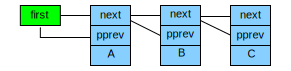
\includegraphics{defer/Linux_hlist}}
\end{center}
\caption{Linux Linear Linked List}
\label{fig:defer:Linux Linear Linked List}
\end{figure}

리눅스의 다른 이중 링크드 리스트인 hlist 는 선형 리스트인데, 이는 헤더로의
포인터만이 필요하지
Figure~\ref{fig:defer:Linux Linear Linked List} 에 보여진 순환 형태의
리스트처럼 두개의 포인터가 필요하진 않습니다.
따라서, hlist 의 사용은 해시 버킷 배열들이나 커다란 해시 테이블에서는 메모리
사용량을 반으로 줄일 수 있습니다.
앞에서와 같이, 이 형태는 다루기가 까다로우므로, hlist 들은
Figure~\ref{fig:defer:Linux Linked List Abbreviated} 에 보인 것과 같은 형태로
간략화 될 겁니다.
\iffalse

Linux's other doubly linked list, the hlist,
is a linear list, which means that
it needs only one pointer for the header rather than the two
required for the circular list, as shown in
Figure~\ref{fig:defer:Linux Linear Linked List}.
Thus, use of hlist can halve the memory consumption for the hash-bucket
arrays of large hash tables.
As before, this notation is cumbersome, so hlists will be abbreviated
in the same way lists are, as shown in
Figure~\ref{fig:defer:Linux Linked List Abbreviated}.
\fi

\begin{figure}[tbp]
{ \scriptsize
\begin{verbatim}
  1 struct foo {
  2   struct hlist_node *list;
  3   int a;
  4   int b;
  5   int c;
  6 };
  7 HLIST_HEAD(head);
  8
  9 /* . . . */
 10
 11 p = kmalloc(sizeof(*p), GFP_KERNEL);
 12 p->a = 1;
 13 p->b = 2;
 14 p->c = 3;
 15 hlist_add_head_rcu(&p->list, &head);
\end{verbatim}
}
\caption{RCU {\tt hlist} Publication}
\label{fig:defer:RCU hlist Publication}
\end{figure}

새로운 원소를 RCU 로 보호되는 hlist 에 공개하는 건
as shown in Figure~\ref{fig:defer:RCU hlist Publication} 에 보여진 것처럼,
순환형 리스트에서 했던 것과 상당히 유사합니다.

앞에서와 같이, line~15 는 예를 들면 락과 같은, 어떤 종류의 동기화 메커니즘으로
보호되어야만 합니다.

RCU 로 보호되는 hlist 를 구독하는 행위 역시 순환형 리스트에서와 비슷합니다:
\iffalse

Publishing a new element to an RCU-protected hlist is quite similar
to doing so for the circular list,
as shown in Figure~\ref{fig:defer:RCU hlist Publication}.

As before, line~15 must be protected by some sort of synchronization
mechanism, for example, a lock.

Subscribing to an RCU-protected hlist is also similar to the
circular list:
\fi

\vspace{5pt}
\begin{minipage}[t]{\columnwidth}
\scriptsize
\begin{verbatim}
  1 rcu_read_lock();
  2 hlist_for_each_entry_rcu(p, q, head, list) {
  3   do_something_with(p->a, p->b, p->c);
  4 }
  5 rcu_read_unlock();
\end{verbatim}
\end{minipage}
\vspace{5pt}

\QuickQuiz{}
	{\tt list\_for\_each\_entry\_rcu()} 에서는 한개면 되었던 포인터가 왜
	{\tt hlist\_for\_each\_entry\_rcu()} 에서는 두개나 넘겨줘야 하는거죠?
	\iffalse

	Why do we need to pass two pointers into
	{\tt hlist\_for\_each\_entry\_rcu()}
	when only one is needed for {\tt list\_for\_each\_entry\_rcu()}?
	\fi
\QuickQuizAnswer{
	hlist 에서는 헤드를 만나는 대신에 NULL 체크를 할 필요가 있기
	때문입니다.
	(하나의 포인터만 사용하는 {\tt hlist\_for\_each\_entry\_rcu()} 를
	한번 구현해 보세요.
	만약 좋은 해결책을 찾는다면, 정말 좋은 일일 겁니다!)
	\iffalse

	Because in an hlist it is necessary to check for
	NULL rather than for encountering the head.
	(Try coding up a single-pointer {\tt hlist\_for\_each\_entry\_rcu()}.
	If you come up with a nice solution, it would be a very good thing!)
	\fi
} \QuickQuizEnd

\begin{table*}[tb]
\begin{center}
\scriptsize
\begin{tabular}{l||l|l|l}
Category  & Publish	& Retract	& Subscribe \\
\hline
\hline
Pointers  & \co{rcu_assign_pointer()}
			& \co{rcu_assign_pointer(..., NULL)}~~
					& \co{rcu_dereference()} \\
\hline
Lists     & \parbox{1.5in}{
		\co{list_add_rcu()} \\
		\co{list_add_tail_rcu()} \\
		\co{list_replace_rcu()} }
			& \co{list_del_rcu()}
					& \co{list_for_each_entry_rcu()}~~~ \\
\hline
Hlists    & \parbox{1.5in}{
		\co{hlist_add_after_rcu()} \\
		\co{hlist_add_before_rcu()}  \\
		\co{hlist_add_head_rcu()} \\
		\co{hlist_replace_rcu()} }
			& \co{hlist_del_rcu()}
					& \co{hlist_for_each_entry_rcu()}~~~~~
\end{tabular}
\end{center}
\caption{RCU Publish and Subscribe Primitives}
\label{tab:defer:RCU Publish and Subscribe Primitives}
\end{table*}

RCU 공개와 구독 기능들의 집합이
Table~\ref{tab:defer:RCU Publish and Subscribe Primitives} 에 ``구독취소'' 또는
철회를 위한 추가적인 기능들과 함께 표시 되어 있습니다.

\co{list_replace_rcu()}, \co{list_del_rcu()},
\co{hlist_replace_rcu()}, and \co{hlist_del_rcu()}
API 들이 복잡도를 더함을 알아두세요.
교체되거나 삭제된 데이터 원소를 메모리에서 해제하는데 안전한 시점은 언제일까요?
자세히 들어가서, 모든 읽기 작업들이 특정 데이터 원소로의 레퍼런스들을
해제한 시점을 어떻게 하면 알 수 있을까요?

이 질문들은 다음의 섹션에서 다루어집니다.
\iffalse

The set of RCU publish and subscribe primitives are shown in
Table~\ref{tab:defer:RCU Publish and Subscribe Primitives},
along with additional primitives to ``unpublish'', or retract.

Note that the \co{list_replace_rcu()}, \co{list_del_rcu()},
\co{hlist_replace_rcu()}, and \co{hlist_del_rcu()}
APIs add a complication.
When is it safe to free up the data element that was replaced or
removed?
In particular, how can we possibly know when all the readers
have released their references to that data element?

These questions are addressed in the following section.
\fi

\subsubsection{Wait For Pre-Existing RCU Readers to Complete}
\label{sec:defer:Wait For Pre-Existing RCU Readers to Complete}

가장 기본적인 형태에서, RCU 는 일들이 끝나기를 기다리는 방법입니다.
물론, RCU 외에도 일들이 끝나길 기다리는 훌륭한 방법들이 여럿 있는데, 레퍼런스
카운트, reader-writer lock, 이벤트 등등이 포함됩니다.
RCU 의 커다란 장점은 각각의 (대략) 20,000 개의 서로 다른 일들을 명시적으로 그
모든 것들을 각각 정보를 쫓아가지 않고, 성능 하락, 확장성 제한, 복잡한 데드락
시나리오, 그리고 명시적으로 정보 쫓는 방법에서 필연적인 메모리 누수 문제들을
걱정할 필요 없이 기다릴 수 있다는 겁니다.
\iffalse

In its most basic form, RCU is a way of waiting for things to finish.
Of course, there are a great many other ways of waiting for things to
finish, including reference counts, reader-writer locks, events, and so on.
The great advantage of RCU is that it can wait for each of
(say) 20,000 different things without having to explicitly
track each and every one of them, and without having to worry about
the performance degradation, scalability limitations, complex deadlock
scenarios, and memory-leak hazards that are inherent in schemes
using explicit tracking.
\fi

RCU 의 경우에, 기다려지고 있는 일들은 ``RCU read-side 크리티컬 섹션'' 이라
불립니다.
하나의 RCU read-side 크리티컬 섹션은 \co{rcu_read_lock()} 함수로 시작되고, 그에
연관되는 \co{rcu_read_unlock()} 함수로 종료됩니다.
RCU read-side 크리티컬 섹션들은 중첩될 수 있고, 어떤 코드든 그 코드가
명시적으로 블락하거나 잠들지 않는 한 (SRCU~\cite{PaulEMcKenney2006c} 라고
불리는 특별한 형태의 RCU 가 SRCU read-side 크리티컬 섹션 내에서의 일반적인
잠들기를 가능하게 하긴 하지만), 그 안에 얼마든지 들어갈 수 있습니다.
이런 규칙에 동의한다면, 코드에서 원하는 부분이라면 \emph{어떤 부분이든}
완료되기를 기다리는데에 RCU 를 사용할 수 있습니다.
\iffalse

In RCU's case, the things waited on are called
``RCU read-side critical sections''.
An RCU read-side critical section starts with an
\co{rcu_read_lock()} primitive, and ends with a corresponding
\co{rcu_read_unlock()} primitive.
RCU read-side critical sections can be nested, and may contain pretty
much any code, as long as that code does not explicitly block or sleep
(although a special form of RCU called SRCU~\cite{PaulEMcKenney2006c}
does permit general sleeping in SRCU read-side critical sections).
If you abide by these conventions, you can use RCU to wait for \emph{any}
desired piece of code to complete.
\fi

RCU 는 언제 이런 기다리는 중인 일들이 종료되었는지를 간접적으로 판단해내는
것으로 이 기능을 구현합니다~\cite{PaulEMcKenney2007whatisRCU,
PaulEMcKenney2007PreemptibleRCU}.
\iffalse

RCU accomplishes this feat by indirectly determining when these
other things have finished~\cite{PaulEMcKenney2007whatisRCU,
PaulEMcKenney2007PreemptibleRCU}.
\fi

\begin{figure}[tb]
\begin{center}
\resizebox{3in}{!}{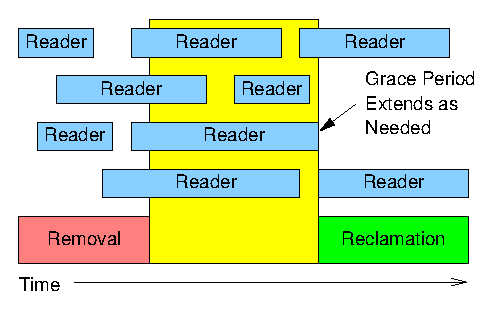
\includegraphics{defer/GracePeriodGood}}
\end{center}
\caption{Readers and RCU Grace Period}
\label{fig:defer:Readers and RCU Grace Period}
\end{figure}

자세히 말하자면,
Figure~\ref{fig:defer:Readers and RCU Grace Period} 에 보여진 것처럼, RCU 는
전부터 존재했던 RCU read-side 크리티컬 섹션들이 그 크리티컬 센션들에서 수행되는
메모리 오퍼레이션 등이 완전히 끝나기를 기다리는 한가지 방법입니다.
하지만, 주어진 grace period 의 시작 후에 시작된 RCU read-side 크리티컬 섹션들은
그 grace period 의 종료 이후까지 수행될 수도 있음을 기억해 두십시오.

다음의 슈도코드는 RCU 를 이용해 읽기 작업들을 기다리는 알고리즘들의 기본적
형태를 보입니다:
\iffalse

In particular, as shown in
Figure~\ref{fig:defer:Readers and RCU Grace Period},
RCU is a way of
waiting for pre-existing RCU read-side critical sections to completely
finish, including memory operations executed by those critical sections.
However, note that RCU read-side critical sections
that begin after the beginning
of a given grace period can and will extend beyond the end of that grace
period.

The following pseudocode shows the basic form of algorithms that use
RCU to wait for readers:
\fi

\begin{enumerate}
\item	링크드 리스트에서 한 원소를 바꿔치기 하거나 하는 식으로 변경을
	만듭니다.
\item	전부터 존재했던 RCU read-side 크리티컬 섹션들이 완전히 종료되길
	기다립니다 (예를 들어, \co{synchronize_rcu()} 기능을 이용해서).
	여기서의 핵심은 뒤이어지는 RCU read-side 크리티컬 섹션들은 이제는
	제거된 원소로의 레퍼런스를 얻을 수 없다는 점입니다.
\item	예를 들어 앞서 교체된 원소를 메모리에서 해제하는 식으로 정리를 합니다.
\iffalse

\item	Make a change, for example, replace an element in a linked list.
\item	Wait for all pre-existing RCU read-side critical sections to
	completely finish (for example, by using the
	\co{synchronize_rcu()} primitive).
	The key observation here is that subsequent RCU read-side critical
	sections have no way to gain a reference to the newly removed
	element.
\item	Clean up, for example, free the element that was replaced above.
\fi
\end{enumerate}

\begin{figure}[tbp]
{ \scriptsize
\begin{verbatim}
  1 struct foo {
  2   struct list_head *list;
  3   int a;
  4   int b;
  5   int c;
  6 };
  7 LIST_HEAD(head);
  8
  9 /* . . . */
 10
 11 p = search(head, key);
 12 if (p == NULL) {
 13   /* Take appropriate action, unlock, & return. */
 14 }
 15 q = kmalloc(sizeof(*p), GFP_KERNEL);
 16 *q = *p;
 17 q->b = 2;
 18 q->c = 3;
 19 list_replace_rcu(&p->list, &q->list);
 20 synchronize_rcu();
 21 kfree(p);
\end{verbatim}
}
\caption{Canonical RCU Replacement Example}
\label{fig:defer:Canonical RCU Replacement Example}
\end{figure}

Figure~\ref{fig:defer:Canonical RCU Replacement Example} 에 보여진 코드 조각은
Section~\ref{sec:defer:Publish-Subscribe Mechanism} 에서 가져와진 것으로, 이
프로세스를 보여주는데,  필드 \co{a} 는 검색을 위한 키로 사용됩니다.

Line~19, 20, 21 은 앞에서 이야기한 세개의 스텝을 보입니다.
Line~16-19 이 RCU (``read-copy update'') 에 그 이름을 줍니다: 동시의
\emph{read} 를 허용하면서, line~16 은 \emph{copy} 를 하고 line~17-19 에서 실제
\emph{update} 를 합니다.
\iffalse

The code fragment shown in
Figure~\ref{fig:defer:Canonical RCU Replacement Example},
adapted from those in Section~\ref{sec:defer:Publish-Subscribe Mechanism},
demonstrates this process, with field \co{a} being the search key.

Lines~19, 20, and 21 implement the three steps called out above.
Lines~16-19 gives RCU (``read-copy update'') its name: while permitting
concurrent \emph{reads}, line~16 \emph{copies} and lines~17-19
do an \emph{update}.
\fi

Section~\ref{sec:defer:Introduction to RCU} 에서 이야기된 것처럼,
\co{synchronize_rcu()} 기능은 매우 간단할 수 있습니다 (``장난감'' RCU 구현을 더
보기 위해선 Section~\ref{sec:defer:``Toy'' RCU Implementations} 을 참고하시기
바랍니다).
하지만, 상품 수준의 구현들은 복잡하고 희귀한 경우들을 처리해야 하고 강력한
최적화를 포함해야 하는데, 둘 다 상당한 복잡도가 생기게 하고 맙니다.
\co{synchronize_rcu()} 의 간단한 개념적 구현이 있음을 알게 된 건 좋지만, 다른
질문들이 남습니다.
예를 들어, RCU 읽기 작업들은 동시에 업데이트 되는 리스트를 돌아다니면서 정확히
뭘 보게 되는 걸까요?
이 질문을 다음 섹션에서 다루도록 합니다.
\iffalse

As discussed in Section~\ref{sec:defer:Introduction to RCU},
the \co{synchronize_rcu()} primitive can be quite simple
(see Section~\ref{sec:defer:``Toy'' RCU Implementations}
for additional ``toy'' RCU implementations).
However, production-quality implementations must deal with
difficult corner cases and also incorporate
powerful optimizations, both of which result in significant complexity.
Although it is good to know that there is a simple conceptual
implementation of \co{synchronize_rcu()}, other questions remain.
For example, what exactly do RCU
readers see when traversing a concurrently updated list?
This question is addressed in the following section.
\fi

\subsubsection{Maintain Multiple Versions of Recently Updated Objects}
\label{sec:defer:Maintain Multiple Versions of Recently Updated Objects}

이 섹션은 RCU 가 동기화로부터 자유로운 읽기 작업들을 허용하기 위해 리스트의
여러 버전들을 어떻게 관리하는지 보입니다.
주어진 읽기 쓰레드에 의해 레퍼런스될 수도 있는 원소가 해당 읽기 쓰레드가 자신의
RCU read-side 크리티컬 섹션을 유지하고 있는 동안에도 손상되지 않은채로 어떻게
유지될 수 있는지를 두개의 예제로 보일 겁니다.
첫번째 예제는 리스트 원소의 삭제를 보이고, 두번째 예제는 원소의 교체를 보이도록
하겠습니다.
\iffalse

This section demonstrates how RCU maintains multiple versions of
lists to accommodate synchronization-free readers.
Two examples are presented showing how an element
that might be referenced by a given reader must remain intact
while that reader remains in its RCU read-side critical section.
The first example demonstrates deletion of a list element,
and the second example demonstrates replacement of an element.
\fi

\paragraph{Example 1: Maintaining Multiple Versions During Deletion}
\label{sec:defer:Example 1: Maintaining Multiple Versions During Deletion}

이제 Section~\ref{sec:defer:Introduction to RCU} 에서의 원소 삭제 예제를 다시
들여다 보되, 이번에는 그 아래의 RCU 에 있는 기본적인 개념에 대한 확실한 이해와
함께입니다.
이 새로운 버전의 삭제 예제를 시작하기 위해,
Figure~\ref{fig:defer:Canonical RCU Replacement Example} 의 line~11-21 을
다음과 같이 보이게 수정할 겁니다:
\iffalse

We can now revisit the deletion example from
Section~\ref{sec:defer:Introduction to RCU},
but now with the benefit of a firm understanding of the fundamental
concepts underlying RCU.
To begin this new version of the deletion example,
we will modify lines~11-21 in
Figure~\ref{fig:defer:Canonical RCU Replacement Example}
to read as follows:
\fi

\vspace{5pt}
\begin{minipage}[t]{\columnwidth}
\scriptsize
\begin{verbatim}
  1 p = search(head, key);
  2 if (p != NULL) {
  3   list_del_rcu(&p->list);
  4   synchronize_rcu();
  5   kfree(p);
  6 }
\end{verbatim}
\end{minipage}
\vspace{5pt}

\begin{figure}[tb]
\begin{center}
\resizebox{3in}{!}{\includegraphics{defer/RCUDeletion}}
\end{center}
\caption{RCU Deletion From Linked List}
\label{fig:defer:RCU Deletion From Linked List}
\end{figure}

이 코드는
Figure~\ref{fig:defer:RCU Deletion From Linked List} 에 보인 것처럼 리스트를
업데이트 할 겁니다.
각 원소의 세개의 숫자는 필드 \co{a}, \co{b}, \co{c} 의 값들을 각각 나타냅니다.
빨간색으로 칠해진 원소들은 RCU 읽기 쓰레드들이 그것들로의 레퍼런스를 가질 수
있음을 나타내는데, 따라서 다이어그램의 꼭대기에 있는 최초의 상태에서는 모든
원소들이 빨간색으로 칠해져 있습니다.
뒤로의 포인터들과 리스트의 tail 로부터 head 로의 링크는 가독성을 위해 삭제해
둔점을 알아 두시기 바랍니다.
\iffalse

This code will update the list as shown in
Figure~\ref{fig:defer:RCU Deletion From Linked List}.
The triples in each element represent the values of fields \co{a},
\co{b}, and \co{c}, respectively.
The red-shaded elements
indicate that RCU readers might be holding references to them,
so in the initial state at the top of the diagram, all elements
are shaded red.
Please note that
we have omitted the backwards pointers and the link from the tail
of the list to the head for clarity.
\fi

Line~3 에서의 \co{list_del_rcu()} 가 완료된 후에, \co{5,6,7}~원소는
Figure~\ref{fig:defer:RCU Deletion From Linked List} 의 두번째 줄에 보여진
것처럼 리스트에서 삭제되어 있습니다.
읽기 쓰레드들은 업데이트 쓰레드들과 직접적으로 동기화를 하지 않으므로, 읽기
쓰레드들은 동시에 이 리스트를 스캔 하고 있을 수 있습니다.
이런 동시의 읽기 쓰레드들은 이번에 삭제된 원소를 타이밍에 따라서는 볼수도, 보지
않을 수도 있습니다.
하지만, 이번에 삭제된 원소로의 포인터를 가져온 후에 한동안 지연된 (ex:
인터럽트나 ECC 메모리 에러, 또는 \co{CONFIG_PREEMPT_RT} 커널에서라면 preemption
으로 인해서) 읽기 쓰레드들은 이 삭제로부터 상당한 시간이 흐른 후에도 이
리스트의 과거 버전을 보게 될 수도 있습니다.
따라서, 이 리스트의 두개의 버전이 있는 셈인데, 하나는 \co{5,6,7} 원소를 가지고
있고 또다른 하나는 가지고 있지 않습니다.
이 그림에서 두번째 줄의 \co{5,6,7}~원소는 노란색으로 칠해져 있는데, 오래된 읽기
쓰레드들은 여전히 레퍼런스를 가지고 있을 수 있지만, 새로 시작된 읽기 쓰레드들은
그로의 레퍼런스를 얻을 수 없음을 의미합니다.
\iffalse

After the \co{list_del_rcu()} on
line~3 has completed, the \co{5,6,7}~element
has been removed from the list, as shown in the second row of
Figure~\ref{fig:defer:RCU Deletion From Linked List}.
Since readers do not synchronize directly with updaters,
readers might be concurrently scanning this list.
These concurrent readers might or might not see the newly removed element,
depending on timing.
However, readers that were delayed (e.g., due to interrupts, ECC memory
errors, or, in \co{CONFIG_PREEMPT_RT} kernels, preemption)
just after fetching a pointer to the newly removed element might
see the old version of the list for quite some time after the
removal.
Therefore, we now have two versions of the list, one with element
\co{5,6,7} and one without.
The \co{5,6,7}~element in the second row of the figure is now
shaded yellow, indicating
that old readers might still be referencing it, but that new
readers cannot obtain a reference to it.
\fi

읽기 쓰레드들은 각자의 RCU read-side 크리티컬 섹션들에서 빠져나온 후에는
element~\co{5,6,7} 로의 레퍼런스를 얻을 수 없음을 기억하기 바랍니다.
따라서, 일단 line~4 에서의 \co{synchronize_rcu()} 가 완료되면, 모든 앞서
존재하던 읽기 쓰레드들은 완료된 것이 보장되므로, 이 원소를 레퍼런스 하는 읽기
쓰레드들은 존재할 수 없어지는데
Figure~\ref{fig:defer:RCU Deletion From Linked List} 의 세번째 줄에 녹색으로
색칠됨으로써 이 상황이 나타내어져 있습니다.

이 시점에서, \co{5,6,7}~원소는
Figure~\ref{fig:defer:RCU Deletion From Linked List} 의 마지막 줄에 나타나
있듯이 안전하게 메모리 해제될 수 있습니다.
이 시점에서, 원소~\co{5,6,7} 의 삭제가 완료되었습니다.
다음 섹션에서는 교체를 다룹니다.
\iffalse

Please note that readers are not permitted to maintain references to
element~\co{5,6,7} after exiting from their RCU read-side
critical sections.
Therefore,
once the \co{synchronize_rcu()} on
line~4 completes, so that all pre-existing readers are
guaranteed to have completed,
there can be no more readers referencing this
element, as indicated by its green shading on the third row of
Figure~\ref{fig:defer:RCU Deletion From Linked List}.
We are thus back to a single version of the list.

At this point, the \co{5,6,7}~element may safely be
freed, as shown on the final row of
Figure~\ref{fig:defer:RCU Deletion From Linked List}.
At this point, we have completed the deletion of
element~\co{5,6,7}.
The following example covers replacement.
\fi

\paragraph{Example 2: Maintaining Multiple Versions During Replacement}
\label{sec:defer:Example 2: Maintaining Multiple Versions During Replacement}

교체의 예제 설명을 위해, 여기
Figure~\ref{fig:defer:Canonical RCU Replacement Example} 예제의
마지막 몇줄의 코드를 붙여넣습니다:
\iffalse

To start the replacement example,
here are the last few lines of the
example shown in
Figure~\ref{fig:defer:Canonical RCU Replacement Example}:
\fi

\vspace{5pt}
\begin{minipage}[t]{\columnwidth}
\scriptsize
\begin{verbatim}
  1 q = kmalloc(sizeof(*p), GFP_KERNEL);
  2 *q = *p;
  3 q->b = 2;
  4 q->c = 3;
  5 list_replace_rcu(&p->list, &q->list);
  6 synchronize_rcu();
  7 kfree(p);
\end{verbatim}
\end{minipage}
\vspace{5pt}

\begin{figure}[tbp]
\begin{center}
\resizebox{2.7in}{!}{\includegraphics{defer/RCUReplacement}}
\end{center}
\caption{RCU Replacement in Linked List}
\label{fig:defer:RCU Replacement in Linked List}
\end{figure}

리스트의 초기의 상태는 \co{p} 포인터를 포함해서 삭제 예제와 동일한데,
Figure~\ref{fig:defer:RCU Replacement in Linked List} 의 첫번째 줄에 보여져
있습니다.

앞에서와 마찬가지로, 각 원소의 세개의 숫자는 필드 \co{a}, \co{b}, \co{c} 를
각각 나타냅니다.
빨간 원소들은 읽기 쓰레드들에 의해 레퍼런스 될 수도 있고, 읽기
쓰레드들은 업데이트 쓰레드들과 직접 동기화를 하지 않기 때문에 읽기
쓰레드들은 이 전체 교체 프로세스와 동시에 수행될 수 있습니다.
이번에도 뒤쪽으로의 포인터들과 리스트의 tail 에서 head 로의 링크는 가독성을
위해 제거되었음을 참고 바랍니다.
\iffalse

The initial state of the list, including the pointer \co{p},
is the same as for the deletion example, as shown on the
first row of
Figure~\ref{fig:defer:RCU Replacement in Linked List}.

As before,
the triples in each element represent the values of fields \co{a},
\co{b}, and \co{c}, respectively.
The red-shaded elements might be referenced by readers,
and because readers do not synchronize directly with updaters,
readers might run concurrently with this entire replacement process.
Please note that
we again omit the backwards pointers and the link from the tail
of the list to the head for clarity.
\fi

아래의 글은 \co{5,6,7} 원소를 \co{5,2,3} 으로 모든 읽기 쓰레드가 이 두 값들 중
하나만 보도록 하면서 어떻게 교체해야 하는지 설명합니다.

Line~1 은 교체할 원소를 \co{kmalloc()} 해서
Figure~\ref{fig:defer:RCU Replacement in Linked List} 의 두번째 줄에 보여진
것과 같은 상태가 만들어지게 합니다.
이 시점에서는, 어떤 릭기 쓰레드도 이 새로 만들어진 원소로의 레퍼런스를 가질 수
없고 (녹색 색깔로 이를 나타냅니다), 이 원소는 아직 초기화되지 않았습니다
(물음표로 나타내어집니다).
\iffalse

The following text describes how to replace the \co{5,6,7} element
with \co{5,2,3} in such a way that any given reader sees one of these
two values.

Line~1 \co{kmalloc()}s a replacement element, as follows,
resulting in the state as shown in the second row of
Figure~\ref{fig:defer:RCU Replacement in Linked List}.
At this point, no reader can hold a reference to the newly allocated
element (as indicated by its green shading), and it is uninitialized
(as indicated by the question marks).
\fi

Line~2 에서는 예전 원소의 값을 새 원소로 복사해서
Figure~\ref{fig:defer:RCU Replacement in Linked List} 의 세번째 줄에 보여진
상태를 만듭니다.
이 새로 만들어진 원소는 여전히 읽기 쓰레드들에 의해 레퍼런스될 수는 없지만,
이제 초기화는 되었습니다.

Line~3 는
Figure~\ref{fig:defer:RCU Replacement in Linked List} 의 네번째 줄에 보여진
것처럼 \co{q->b} 를 값 ``2'' 로, 그리고 line~4 는 \co{q->c} 를 값 ``3'' 으로
바꿉니다.
\iffalse

Line~2 copies the old element to the new one, resulting in the
state as shown in the third row of
Figure~\ref{fig:defer:RCU Replacement in Linked List}.
The newly allocated element still cannot be referenced by readers, but
it is now initialized.

Line~3 updates \co{q->b} to the value ``2'', and
line~4 updates \co{q->c} to the value ``3'', as shown on the fourth row of
Figure~\ref{fig:defer:RCU Replacement in Linked List}.
\fi

이제, line~5 는 교체를 행해서 새 원소가 읽혀질 수 있게
만드는데, 따라서
Figure~\ref{fig:defer:RCU Replacement in Linked List} 의 다섯번째 줄에
빨간색으로 칠해져 있습니다.
이 시점에서는 앞에서와 같이, 두가지 버전의 리스트가 존재합니다.
전부터 있던 읽기 쓰레드들은 \co{5,6,7} 원소를 볼 수 있지만 (따라서
노란색으로 칠해져 있습니다), 새 읽기 쓰레드들은 그대신 \co{5,2,3} 원소를
볼겁니다.
하지만 어떤 읽기 쓰레드들이든 제대로 형태를 갖춘 리스트만을 볼 것이 보장됩니다.
\iffalse

Now, line~5 does the replacement, so that the new element is
finally visible to readers, and hence is shaded red, as shown on
the fifth row of
Figure~\ref{fig:defer:RCU Replacement in Linked List}.
At this point, as shown below, we have two versions of the list.
Pre-existing readers might see the \co{5,6,7} element (which is
therefore now shaded yellow), but
new readers will instead see the \co{5,2,3} element.
But any given reader is guaranteed to see some well-defined list.
\fi

Line~6 의 \co{synchronize_rcu()} 가 리턴한 후에는, grace period 는 지나갔고,
따라서 \co{list_replace_rcu()} 전에 시작된 모든 읽기는 완료된 상태입니다.
특히, \co{5,6,7} 원소로의 레퍼런스를 가지고 있는 모든 읽기 쓰레드들은 각자의
RCU read-side 크리티컬 섹션들을 빠져나왔음이 보장되고, 따라서 레퍼런스를
계속해서 잡고 있을 수 없습니다.
따라서, 과거의 원소로의 레퍼런스를 여전히 잡고 있는 읽기 쓰레드는 더이상 있을
수 없는데, 이 상황이
Figure~\ref{fig:defer:RCU Replacement in Linked List} 의 여섯번째 줄에
초록색으로 나타내어져 있습니다.
읽기 쓰레드들의 관점에서 리스트의 단일 버전만이 존재하는데, 예전 원소는 새
원소로 바뀌어 있습니다.
\iffalse

After the \co{synchronize_rcu()} on line~6 returns,
a grace period will have elapsed, and so all reads that started before the
\co{list_replace_rcu()} will have completed.
In particular, any readers that might have been holding references
to the \co{5,6,7} element are guaranteed to have exited
their RCU read-side critical sections, and are thus prohibited from
continuing to hold a reference.
Therefore, there can no longer be any readers holding references
to the old element, as indicated its green shading in the sixth row of
Figure~\ref{fig:defer:RCU Replacement in Linked List}.
As far as the readers are concerned, we are back to having a single version
of the list, but with the new element in place of the old.
\fi

Line~7 에서의 \co{kfree()} 후에 이 리스트는
Figure~\ref{fig:defer:RCU Replacement in Linked List} 의 마지막 줄에 보여진
것처럼 됩니다.

RCU 는 교체의 경우에 의해서 이름지어졌다는 사실에도 불구하고, 리눅스 커널
안에서의 RCU 사용예의 대다수는
Section~\ref{sec:defer:Maintain Multiple Versions of Recently Updated Objects}.
의 간단한 삭제의 케이스에 기반해 있습니다.
\iffalse

After the \co{kfree()} on line~7 completes, the list will
appear as shown on the final row of
Figure~\ref{fig:defer:RCU Replacement in Linked List}.

Despite the fact that RCU was named after the replacement case,
the vast majority of RCU usage within the Linux kernel relies on
the simple deletion case shown in
Section~\ref{sec:defer:Maintain Multiple Versions of Recently Updated Objects}.
\fi

\paragraph{Discussion}
\label{sec:defer:Discussion}

이 예제들은 모든 업데이트 오퍼레이션들에 뮤텍스가 잡혀 있다고 가정을 하고
있는데, 이 말은 한번에 리스트의 버전은 최대 두개까지만 존재할 수 있음을
의미합니다.
\iffalse

These examples assumed that a mutex was held across the entire
update operation, which would mean that there could be at most two
versions of the list active at a given time.
\fi

\QuickQuiz{}
	리스트의 버전이 두개보다 많을 수 있도록 하기 위해서는 삭제 예제를
	어떻게 수정해야 할까요?
	\iffalse

	How would you modify the deletion example to permit more than two
	versions of the list to be active?
	\fi
\QuickQuizAnswer{
	이를 가능하게 하는 한가지 방법은
	Figure~\ref{fig:defer:Concurrent RCU Deletion} 에 보인 것처럼 하는
	것입니다.
	\iffalse

	One way of accomplishing this is as shown in
	Figure~\ref{fig:defer:Concurrent RCU Deletion}.
	\fi

\begin{figure}[htbp]
{ \centering
\begin{verbatim}
  1 spin_lock(&mylock);
  2 p = search(head, key);
  3 if (p == NULL)
  4   spin_unlock(&mylock);
  5 else {
  6   list_del_rcu(&p->list);
  7   spin_unlock(&mylock);
  8   synchronize_rcu();
  9   kfree(p);
 10 }
\end{verbatim}
}
\caption{Concurrent RCU Deletion}
\label{fig:defer:Concurrent RCU Deletion}
\end{figure}

	이 코드는 여러개의 동시에 수행되는 삭제 작업들이 \co{synchronize_rcu()}
	에서 기다리게 될수도 있음을 의미합니다.
	\iffalse

	Note that this means that multiple concurrent deletions might be
	waiting in \co{synchronize_rcu()}.
	\fi
} \QuickQuizEnd

\QuickQuiz{}
	어떤 시점에 하나의 리스트는 RCU 버전들을 몇개까지 가질 수 있을까요?
	\iffalse

	How many RCU versions of a given list can be
	active at any given time?
	\fi
\QuickQuizAnswer{
	동기화 설계에 따라 달라집니다.
	업데이트를 보호하는 세마포어가 grace period 에 걸쳐 잡혀 있다면, 옛날
	버전과 새로운 버전, 최대 두개의 버전이 있을 수 있을 겁니다.

	하지만, 검색, 업데이트, 그리고 \co{list_replace_rcu()} 만이 락으로
	보호되고 있어서
	Figure~\ref{fig:defer:Concurrent RCU Deletion} 보인 코드에서처럼
	\co{synchronize_rcu()} 가 락의 바깥에 있다고 생각해 봅시다.
	더 나아가서 수많은 쓰레드들이 거의 동시에 RCU 교체 기능을 수행했고, 이
	읽기 쓰레드들은 또한 데이터 구조를 계속해서 지나다니고 있다고 생각해
	봅시다.
	\iffalse

	That depends on the synchronization design.
	If a semaphore protecting the update is held across the grace period,
	then there can be at most two versions, the old and the new.

	However, suppose that only the search, the update, and the
	\co{list_replace_rcu()} were protected by a lock, so that
	the \co{synchronize_rcu()} was outside of that lock, similar
	to the code shown in
	Figure~\ref{fig:defer:Concurrent RCU Deletion}.
	Suppose further that a large number of threads undertook an
	RCU replacement at about the same time, and that readers
	are also constantly traversing the data structure.
	\fi

	그러면 다음과 같은 일련의 이벤트들이
	Figure~\ref{fig:defer:RCU Replacement in Linked List} 의 마지막
	상태로부터 발생할 수 있습니다.
	\iffalse

	Then the following sequence of events could occur, starting from
	the end state of
	Figure~\ref{fig:defer:RCU Replacement in Linked List}:
	\fi

	\begin{enumerate}
	\item	쓰레드~A 가 리스트를 지나가면서 5,2,3 원소로의 레퍼런스를
		얻습니다.
	\item	쓰레드~B 가 5,2,3 원소를 새로운 5,2,4 원소로 교체하고, 자신의
		\co{synchronize_rcu()} 호출이 리턴하길 기다립니다.
	\item	쓰레드~C 가 리스트를 지나가면서 5,2,4 원소로의 레퍼런스를
		얻습니다.
	\item	쓰레드~D 가 5,2,4 원소를 새로운 5,2,5 원소로 교체하고, 자신의
		\co{synchronize_rcu()} 호출이 리턴하길 기다립니다.
	\item	쓰레드~E 가 리스트를 지나가면서 5,2,5 원소로의 레퍼런스를
		얻습니다.
	\item	쓰레드~F 가 5,2,5 원소를 새로운 5,2,6 원소로 교체하고, 자신의
		\co{synchronize_rcu()} 호출이 리턴하길 기다립니다.
	\item	쓰레드~G 가 리스트를 지나가면서 5,2,6 원소로의 레퍼런스를
		얻습니다.
	\item	그리고 앞의 두 스텝들이 빠르게 계속해서 반복되어서 모든
		쓰레드들이 \co{synchronize_rcu()} 호출이 리턴하길 기다립니다.
	\end{enumerate}
	\iffalse

	\item	Thread~A traverses the list, obtaining a reference to
		the 5,2,3 element.
	\item	Thread~B replaces the 5,2,3 element with a new
		5,2,4 element, then waits for its \co{synchronize_rcu()}
		call to return.
	\item	Thread~C traverses the list, obtaining a reference to
		the 5,2,4 element.
	\item	Thread~D replaces the 5,2,4 element with a new
		5,2,5 element, then waits for its \co{synchronize_rcu()}
		call to return.
	\item	Thread~E traverses the list, obtaining a reference to
		the 5,2,5 element.
	\item	Thread~F replaces the 5,2,5 element with a new
		5,2,6 element, then waits for its \co{synchronize_rcu()}
		call to return.
	\item	Thread~G traverses the list, obtaining a reference to
		the 5,2,6 element.
	\item	And the previous two steps repeat quickly, so that all
		of them happen before any of the \co{synchronize_rcu()}
		calls return.
	\end{enumerate}
	\fi

	따라서, 얼마든지 많은 버전들이 존재할 수 있는데, 다만 메모리 크기와
	얼마나 많은 업데이트들이 하나의 grace period 안에 완료될 수 있느냐에 그
	수가 제한됩니다.
	하지만 그렇게 자주 업데이트 되는 데이터 구조체들은 RCU 를 사용하기에
	적합한 후보가 아닐 수 있음을 알아두시기 바랍니다.
	그렇다곤 해도, RCU 는 필요할 때에는 높은 비율의 업데이트를 처리할 수
	있습니다.
	\iffalse

	Thus, there can be an arbitrary number of versions active,
	limited only by memory and by how many updates could be completed
	within a grace period.
	But please note that data structures that are updated so frequently
	probably are not good candidates for RCU.
	That said, RCU can handle high update rates when necessary.
	\fi
} \QuickQuizEnd

이 일련의 이벤트들은 RCU 업데이트들이 어떻게 여러 버전들을 사용해 동시에
수행중인 읽기 작업들에도 불구하고 안전하게 변경을 처리하는지 보입니다.
물론, 일부 알고리즘들은 여러 버전들을 잘 처리하지 못합니다.
그런 알고리즘을 RCU 에 적용하는 테크닉~\cite{PaulEdwardMcKenneyPhD} 들이
있지만, 이것들은 이 섹션의 범위를 넘어섭니다.
\iffalse

This sequence of events shows how RCU updates use multiple versions to safely
carry out changes in presence of concurrent readers.  Of course, some
algorithms cannot gracefully handle multiple versions.  There are techniques
for adapting such algorithms to RCU~\cite{PaulEdwardMcKenneyPhD},
but these are beyond the scope of this section.
\fi

\subsubsection{Summary of RCU Fundamentals}
\label{sec:defer:Summary of RCU Fundamentals}

이 섹션에서는 RCU 기반 알고리즘들의 세가지 기본 컴포넌트들을 설명했습니다:
\iffalse

This section has described the three fundamental components of RCU-based
algorithms:
\fi

\begin{enumerate}
\item	새로운 데이터의 추가를 위한 공개-구독 메커니즘,

\item	전부터 존재했던 RCU 읽기 쓰레드들이 종료되기를 위해 기다리는 방법,
	그리고

\item	동시에 수행중인 RCU 읽기 쓰레드들에 피해를 주거나 지나치게 대기하도록
	만들지 않고 변화를 가할 수 있도록 여러 버전들을 관리하는 방법.
\iffalse

\item	a publish-subscribe mechanism for adding new data,

\item	a way of waiting for pre-existing RCU readers to finish, and

\item	a discipline of maintaining multiple versions to permit
	change without harming or unduly delaying concurrent RCU readers.
\fi
\end{enumerate}

\QuickQuiz{}
	{\tt rcu\_read\_lock()} 과 {\tt rcu\_read\_unlock()} 함수는 스핀하지도
	블락하지도 않는데 어떻게 RCU 업데이트 쓰레드들이 RCU 읽기 쓰레드들을
	대기시킬 수가 있나요?
	\iffalse

	How can RCU updaters possibly delay RCU readers, given that the
	{\tt rcu\_read\_lock()} and {\tt rcu\_read\_unlock()}
	primitives neither spin nor block?
	\fi
\QuickQuizAnswer{
	특정 RCU 업데이터에 의해서 가해진 수정사항은 연관된 CPU 가 해당
	데이터를 포함하는 캐시 라인들을 무효화 하도록 만들 것이고, 동시에
	수행중인 RCU 읽기 쓰레드들을 수행중인 해당 CPU 들이 비싼 캐시 미스를
	마주하도록 만들 것입니다.
	(동시에 수행중인 읽기 쓰레드들에게 비싼 캐시 미스를 만들지 않고 데이터
	구조에 변경을 가할 수 있는 알고리즘을 설계할 수 있을까요?
	또는 뒤따르는 읽기 쓰레드들에게?)
	\iffalse

	The modifications undertaken by a given RCU updater will cause the
	corresponding CPU to invalidate cache lines containing the data,
	forcing the CPUs running concurrent RCU readers to incur expensive
	cache misses.
	(Can you design an algorithm that changes a data structure
	\emph{without}
	inflicting expensive cache misses on concurrent readers?
	On subsequent readers?)
	\fi
} \QuickQuizEnd

이 세개의 RCU 컴포넌트들은 데이터가 동시에 수행되는 읽기 쓰레드들에 상관 없이
업데이트 되도록 하고, 놀랍도록 다양한, 다른 종류의 RCU 기반의 알고리즘들을
구현하는 다른 방법들로 조합될 수 있는데, 그 중 일부는 다음 섹션에서
설명하겠습니다.
\iffalse

These three RCU components
allow data to be updated in face of concurrent readers, and
can be combined in different ways to
implement a surprising variety of different types of RCU-based algorithms,
some of which are described in the following section.
\fi
